% Chapter Template

\chapter{Preliminary Studies} % Main chapter title

\label{Preliminary Studies} % Change X to a consecutive number; for referencing this chapter elsewhere, use \ref{ChapterX}

\lhead{Chapter 5. \emph{Preliminary Studies}} % Change X to a consecutive number; this is for the header on each page - perhaps a shortened title

This chapter contains

%----------------------------------------------------------------------------------------
%	SECTION 1
%----------------------------------------------------------------------------------------
\section{Development Methodology}

TODO

%-----------------------------------
%	SUBSECTION 1
%-----------------------------------
\subsection{Waterfall Model}

The waterfall model is a software development process where each task is performed in a sequential order.
Before moving to the next phase the preceding task needs to be finished.
The progress of the project is seen as flowing downwards through the different phases, hence the name waterfall.
In the original model the phases consisted of seven different tasks:


\begin{enumerate}
\item Requirements specification
\item Design
\item Construction (implementation or coding)
\item Integration
\item Testing and debugging
\item Installation
\item Maintenance
\end{enumerate}

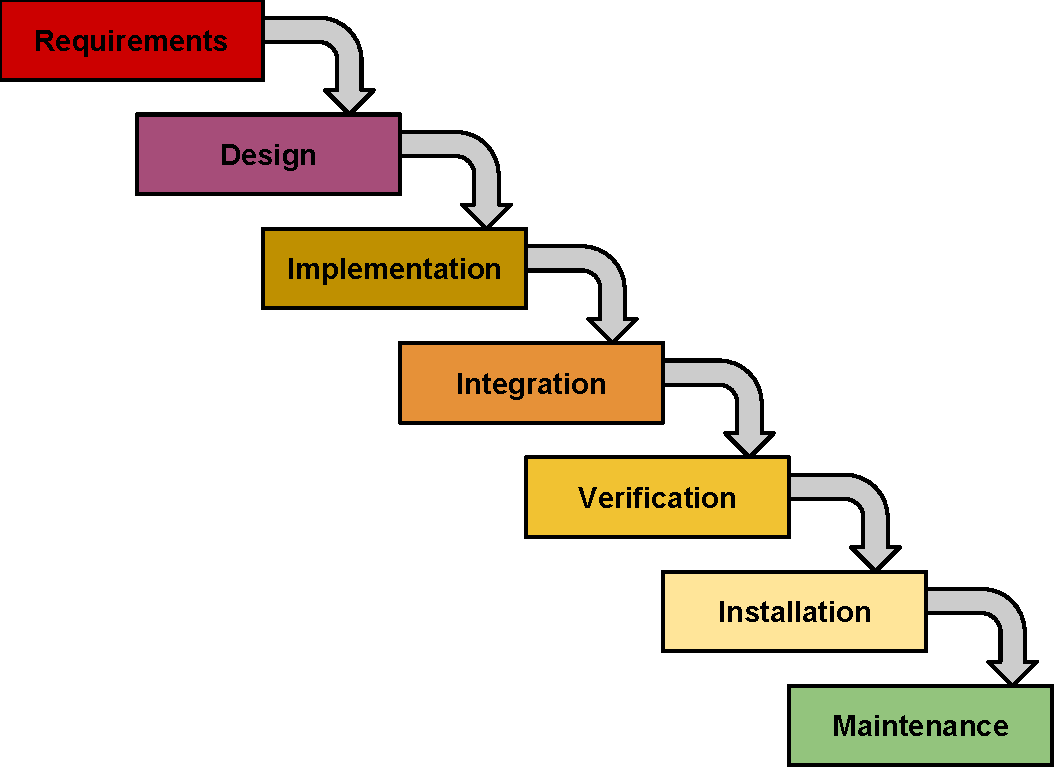
\includegraphics[scale=0.6]{../Figures/Waterfall-model.pdf}

Because each phase needs to be perfected and completed before moving to the next phase, this brings up some difficulties if the requirements were to change during the development process. 
However the model is easily understandable, structured, and disciplined. 
All the phases are divided into different sections, and this makes it easier to understand the progress of the project.
In practice it can be very hard to adapt to this kind of development model. 
It can be hard for a system designer to predict future implementation difficulties of a type of design, hence the design of the system may change during the process.
Another problem is that the customer is not always sure about the system requirements, and often will the customer change them during the development.

%-----------------------------------
%	SUBSECTION 2
%-----------------------------------
\subsection{SCRUM Model}

The SCRUM model is an agile software development process that is iterative and incremental.
It consists of multiple sprints, where a sprint usually lasts from 14-30 days depending on the size of the task.
Each sprint is focusing on a set of concrete goals that are in the sprint backlog.
The sprint backlog consists of tasks that are chosen from the product backlog. 
They are usually chosen in the sprint planning meeting that is performed before each sprint.
The product backlog consists of all the features the product should contain, and is usually made in the initial phase of the project.
It can however be changed and adjusted during the development of the product.
For each day a daily scrum meeting should be performed. 
Usually a scrum meeting consists of getting to know what each person did yesterday, what they will do today and if they are facing any problems.
If there are any problems the Scrum master is responsible to resolve the problem.
After each sprint a sprint review meeting should be held.
An overview of what goals where achieved and which one where not should be made.
The meeting can also consist of a demo of the new features implemented.

%-----------------------------------
%	SUBSECTION 3
%-----------------------------------
\subsection{Conclusion}

We decided to choose the SCRUM model as our development process.	

%----------------------------------------------------------------------------------------
%	SECTION 2
%----------------------------------------------------------------------------------------

\section{Existing Solutions}

This section contains some of the similar existing solutions that are already created.

%-----------------------------------
%	SUBSECTION 1
%-----------------------------------
\subsection{HealthVault}

TODO

%-----------------------------------
%	SUBSECTION 2
%-----------------------------------
\subsection{Open eHealth Foundation}

TODO

%-----------------------------------
%	SUBSECTION 3
%-----------------------------------
\subsection{human/api}

The human API is a platform for human health data. 
They have an API that contains multiple different well defined JSON strings for different kinds of human related data.
Each JSON string contains all the necessary information that is needed to represent each type of health data.
For example heart rate is defined by an id, user id, time, value and unit in the following way:

\begin{verbatim}
{
  "id": "string",
  "userId": "string",
  "time": "date",
  "value": "int",
  "unit": "string"
}
\end{verbatim}

%-----------------------------------
%	SUBSECTION 4
%-----------------------------------
\subsection{Conclusion}

TODO

%----------------------------------------------------------------------------------------
%	SECTION 3
%----------------------------------------------------------------------------------------
\section{Technologies}

This section contains the technologies we used in our prototype.

%-----------------------------------
%	SUBSECTION 1
%-----------------------------------
\subsection{Server}

\textbf{Java}

TODO

\textbf{Spring Framework}

TODO

\textbf{Apache Tomcat}

Apache Tomcat is an implementation of the JSP (JavaServer Pages) and Java Servlet technologies.
It makes it possible to deploy and run a web page with its services on a server.

%-----------------------------------
%	SUBSECTION 3
%-----------------------------------
\subsection{Database}

\textbf{MySQL}

MySQL is one of the most widely used relational database management system.

%-----------------------------------
%	SUBSECTION 4
%-----------------------------------
\subsection{Web Page}

\textbf{HTML5}

HTML is the standard World Wide Web's markup language.
It is used to structure and visualize web pages on the internet.

\textbf{CSS3}

CSS describes the look and format of a document written in HTML.

\textbf{JavaScript}

JavaScript is an interpreted computer programming language that is run in the browser of the user.
It is allowed to make changes in the HTML DOM, interact with the user, control the browser and communicate asynchronously.

\textbf{jQuery}

jQuery is a JavaScript library for manipulating and traversing the HTML DOM.
It also makes it easier to communicate with the server through AJAX.

\textbf{Chart.js}

Chart.js is a JavaScript library for creating graphs and charts.

%-----------------------------------
%	SUBSECTION 5
%-----------------------------------
\subsection{Mobile Technologies}

\textbf{Android SDK}

Android SDK contains the tools necessary for developing, debugging and testing an Android app.

%-----------------------------------
%	SUBSECTION 6
%-----------------------------------
\subsection{Conclusion}

TODO

%----------------------------------------------------------------------------------------
%	SECTION 4
%----------------------------------------------------------------------------------------
\section{Testing}

TODO

%-----------------------------------
%	SUBSECTION 1
%-----------------------------------
\subsection{JUnit}

TODO

%-----------------------------------
%	SUBSECTION 2
%-----------------------------------
\subsection{Conclusion}

%----------------------------------------------------------------------------------------
%	SECTION 5
%----------------------------------------------------------------------------------------

\section{Summary}

TODO
